%% This is file `jasr-template.tex',
%% 
%% Copyright 2019-2023 Elsevier Ltd
%% 
%% This file is part of the 'Elsarticle Bundle'.
%% ---------------------------------------------
%% 
%% It may be distributed under the conditions of the LaTeX Project Public
%% License, either version 1.2 of this license or (at your option) any
%% later version.  The latest version of this license is in
%%    http://www.latex-project.org/lppl.txt
%% and version 1.2 or later is part of all distributions of LaTeX
%% version 1999/12/01 or later.
%% 
%% The list of all files belonging to the 'Elsarticle Bundle' is
%% given in the file `manifest.txt'.
%% 
%% Template article for Elsevier's document class `elsarticle'
%% with harvard style bibliographic references
%%
%% $Id: jasr-template.tex 235 2023-03-14 12:51:44Z rishi $
%%
%% Use the option review to obtain double line spacing
%\documentclass[times,review,preprint,authoryear]{elsarticle}

%% Use the options `twocolumn,final' to obtain the final layout
%% Use longtitle option to break abstract to multiple pages if overfull.
%% For Review pdf (With double line spacing)
%\documentclass[times,twocolumn,review]{elsarticle}
%% For abstracts longer than one page.
%\documentclass[times,twocolumn,review,longtitle]{elsarticle}
%% For Review pdf without preprint line
%\documentclass[times,twocolumn,review,nopreprintline]{elsarticle}
%% Final pdf
\documentclass[times,authoryear]{elsarticle}
\usepackage{microtype}
%%
%\documentclass[times,twocolumn,final,longtitle]{elsarticle}
%%

%%
%% Stylefile to load JASR template
\usepackage{jasr}
\usepackage{framed,multirow}

%% The amssymb package provides various useful mathematical symbols
\usepackage{amssymb}
\usepackage{latexsym}
\usepackage{amsmath}
%% For line numbers
\usepackage[switch]{lineno}
% Following three lines are needed for this document.
% If you are not loading colors or url, then these are
% not required.
\usepackage{url}
\usepackage{xcolor}
\usepackage[ruled,linesnumbered]{algorithm2e}
\usepackage{algorithm,algorithmic}

\newcommand{\And}{\textbf{and~}}
\newcommand{\Or}{\textbf{or~}}
\newcommand{\Xor}{\textbf{xor~}}
\newcommand{\Not}{\textbf{not~}}
\newcommand{\To}{\textbf{to~}}
\newcommand{\DownTo}{\textbf{downto~}}
\newcommand{\True}{\textbf{true~}}
\newcommand{\False}{\textbf{false~}}
\newcommand{\Input}{\item[\textbf{Input:}]}
\renewcommand{\Output}{\item[\textbf{Output:}]}
\newcommand{\Print}{\State \textbf{print~}}
\renewcommand{\Return}{\State \textbf{return~}}

\definecolor{newcolor}{rgb}{.8,.349,.1}

\usepackage[citebordercolor=white]{hyperref}

\journal{Advances in Space Research}

\begin{document}

\verso{Hang Zhou \textit{etal}}

\begin{frontmatter}

	\title{Type the title of your paper, only capitalize first
		word and proper nouns\tnoteref{tnote1}}%
	% \tnotetext[tnote1]{This is an example for title footnote coding.}

	\author[1]{Hang Zhou}
	\ead{12324046@zju.edu.cn}
	\author[1,2]{Tao Meng\corref{cor1}}
	\ead{mengtao@zju.edu.cn}
	\cortext[cor1]{Corresponding author}


	\address[1]{School of Aeronautics and Astronautics, Zhejiang University, Hangzhou, 310027, China}
	\address[2]{Zhejiang Key Laboratory of Micro-nano satellite Research,  Hangzhou, 310027, China}


	%\address[2]{Affiliation 1, Address, City and Postal Code, Country}
	% \affiliation[1]{organization={Affiliation 1},
	%   addressline={Address},
	%   city={City},
	%   postcode={Postal Code},
	%   country={Country}}

	% %\address[2]{Affiliation 2, Address, City and Postal Code, Country}
	% \affiliation[2]{organization={Affiliation 2},
	%   addressline={Address},
	%   city={City},
	%   postcode={Postal Code},
	%   country={Country}}

	% \received{1 May 2013}
	% \finalform{10 May 2013}
	% \accepted{13 May 2013}
	% \availableonline{15 May 2013}
	% \communicated{S. Sarkar}


	\begin{abstract}
		%%%
		wait for edit
		test -- version
		Please type your abstract here, and the rest of the text, figures,
		tables, equations etc. in the main body. Please do not modify LaTeX\
		commands unless you need to modify them and know how to do it.
		%%%%
	\end{abstract}

	\begin{keyword}
		%% MSC codes here, in the form: \MSC code \sep code
		%% or \MSC[2008] code \sep code (2000 is the default)
		%\MSC 41A05\sep 41A10\sep 65D05\sep 65D17
		%% Keywords
		\KWD motiom planning\sep trajectory optimization\sep time-varying obstacles
	\end{keyword}

\end{frontmatter}

%% For linenumbers
% \linenumbers

%% main text
\section{Introduction}
Reconfiguring spacecraft operations is extremely complex, especially when they approach other objects (such as other spacecraft or space debris). These close-proximity operations carry high risks due to potential collisions and the unpredictable behavior of the objects involved. Consequently, a significant amount of research is dedicated to finding effective collision avoidance strategies for spacecraft motion planning. This research explores a variety of algorithms, ranging from traditional astrodynamics methods, such as calculating trajectories from one point to another, to more advanced techniques like model predictive control and artificial potential functions. Although these advanced methods show effectiveness in control, they often struggle with optimization challenges and varying constraints.

In the search for feasible solutions, some researchers have started focusing on sampling-based motion planning techniques, which are widely used in robotics. These techniques are considered capable of providing insights into complex motion planning problems, achieving collision-free path planning in astrodynamics, and adapting to ever-changing and optimization-demanding conditions. The effectiveness of these techniques has been demonstrated in related literature and offers potential methods and directions for safe motion planning of future spacecraft.

\section{Problem Formulation}

\subsection{System Dynamics}

Since spacecraft proximity operations involve significant drift, space-dependent external forces, and rapid temporal scale changes, any feasible solution must comply with dynamic constraints; In this article, the linearized motion of a circular reference orbit with radius $r_{ref}$ about the Earth's gravitational constant $\mu$ is represented using the classic CWH equations. This model provides a first-order approximation for tracking the motion of a spacecraft relative to the rotating target coordinate system. The linearized motion equations for this scenario are given in the target's LVLH frame.
\begin{subequations}
	% \label{eq1}
	\begin{align}
		\delta\ddot{x}-3n_{\mathrm{ref}}^{2}\delta x-2n_{\mathrm{ref}}\delta\dot{y}=\frac{F_{\delta x}}m \\
		\delta\ddot{y}+2n_{\mathrm{ref}}\delta\dot{x}=\frac{F_{\delta y}}m                               \\
		\delta\ddot{z}+n_{\mathrm{ref}}^{2}\delta z=\frac{F_{\delta z}}m
	\end{align}
\end{subequations}

where, $n_{ref} = \sqrt{\frac{\mu}{r^3_{ref}}}$ is the average angular velocity of the reference orbit, $m$ is the mass of the spacecraft, $\boldsymbol{F} = [{F}_{\delta x}, {F}_{\delta y}, {F}_{\delta z}]^\top$ is the thrust on the spacecraft, and $(\delta x, \delta y, \delta z)$ , $(\delta \dot{x}, \delta \dot{y}, \delta \dot{z})$ are the relative position and velocity vectors.

Define the state variable $\boldsymbol{x}$as $[\delta x,\delta y,\delta z,\delta \dot{x}, \delta \dot{y}, \delta \dot{z}]^{\top}$The control variable $\boldsymbol{u}$is the force exerted on the unit mass $\frac{1}{m} \boldsymbol{F}$, and the CWH equation can be described by a linear time invariant (LTI) system

\begin{equation}
	\begin{align}
		\boldsymbol{\dot{x}} = f(\boldsymbol{x},\boldsymbol{u},t) = \boldsymbol{A}\boldsymbol{x}+\boldsymbol{B}\boldsymbol{u}
	\end{align}
\end{equation}

Where the dynamic matrix $\boldsymbol{A}$ and the input matrix $\boldsymbol{B}$ are given by the following formula
\begin{equation}
  \begin{align}
      \boldsymbol{A} = 
      \begin{bmatrix}
       0 &0 &0 &1 &0 &0 \\
       0 &0 &0 &0 &1 &0 \\
       0 &0 &0 &0 &0 &1 \\
       3n_{ref}^2 &0 &0 &0 &2n_{ref} &0 \\
       0 &0 &0 &-2n_{ref} &0 &0 \\
       0 &0 &-n_{ref}^2 &1 &0 &0
      \end{bmatrix}
      ,\boldsymbol{B} = 
      \begin{bmatrix}
      0 &0 &0 \\
      0 &0 &0 \\
      0 &0 &0 \\
      1 &0 &0 \\
      0 &1 &0 \\
      0 &0 &1
      \end{bmatrix}
  \end{align}
\end{equation}

\subsection{time-varying programming problems}

Aiming at the problem of tracking spacecraft maneuvering towards a single target with time-varying obstacles in a well-defined circular orbit and considering the space-time motion planning problem with unbounded arrival time, we aim to minimize the arrival time under given constraints by adding a time latitude to the state space. We get the space-time state space $\mathcal{Q} = \mathcal{X} \times \mathcal{T}$, where $\mathcal{X} \subset \mathbb{R}^3$ Is the configuration state space,$\mathcal{T}$is the time state space, and $\mathcal{Q}$can be unbounded in time. Let $\mathcal{Q}_{free}\in \mathcal{Q}$ be the collision-free subset of the state, and $Q_{start}$be the initial state, $\mathcal{Q}_{goal} = \mathcal{X}_{goal} \times \mathcal{T}_{goal}$is the target region, and in the following work, the trajectory of the obstacle is assumed to be completely known
Therefore, the planning problem can be described as finding a path solution that avoids time-varying obstacles in the shortest possible time given the initial state $q_{start}(t_{start})$, the target region or the target state $x_{goal} \in \mathcal{X}_{goal}$

\begin{equation}
  \begin{align}
    \label{problem}
    &\min \quad \int_{t_{start}}^{t_{goal}}1dt \\
    &s.t. \quda x(t_{init}) = x_{init} \\
    &\dot{\boldsymbol{x}}(t) = \boldsymbol{A}\boldsymbol{x}+\boldsymbol{B}\boldsymbol{u}\\
    & \boldsymbol{x}(t) \in \mathcal{X}_{free},t \in [t_{init},t_{final}]
  \end{align}
\end{equation}


\section{Main result}

\subsection{Path generation based on TubeST-RRTstar}

The TubeST-RRT* algorithm is an improved version of RRT* Connect, modifying the sampling function, steer function, find nearest function and rewiring function, and setting the motion check function for the spacecraft's motion dynamics.Considering the time-varying information of obstacles and the flight corridor with added nodes, we ensure that the generated trajectory is safe and collision-free during subsequent trajectory optimization. 

RRT* Connect algorithm is an asymptotically optimal bidirectional sampling method widely used in robot path planning with obstacle avoidance constraints. The core idea of the RRT method is to randomly sample in the state space to obtain a series of path nodes and directed edges from the parent node to the child node, forming a search tree $\mathcal{T}_{tree }$. To address planning problems in environments with time-varying obstacles, the Tube-ST-RRT* algorithm is proposed. This algorithm first adds a time dimension to the state space and samples the node times to obtain nodes that meet the time-varying constraints. Secondly, during the node sampling process, a radius variable is sampled to ensure that the node is collision-free within a spherical region of that radius. The final result is a sequence of nodes $\boldsymbol{s} = [\boldsymbol{s_{0}},\boldsymbol{s}_{1}\dots{},\boldsymbol{s}_{n}]$, each containing information on position, velocity, time, and the radius of the maximum collision-free spherical region.

The algorithmic details of Tube-ST-RRT* are provided in Algorithms \ref{alg:algorithm1}. In addition to $\mathcal{S}, q_{start}, \mathcal{X}{goal}, d$, the planning termination condition $ptc$, the probability of sampling a new goal $p_{goal} \in \left (0, 1 \right ]$, and the time limit $t_{\max} \in \left (0, \infty \right]$ are also required. The basic framework is similar to RRT-Connect.

\begin{algorithm}[H]
	\label{alg:algorithm1}
	\caption{TubeST-RRT*}
	\begin{algorithmic}[1]
		\Input{$\mathcal{X},q_{start},x_{goal},p_{goal},range\_d,Param,ptc$  }
		\Output{$Soulution$}

		\STATE{$r_{start} \gets FindMaxRadius(s_{start})$}
		\STATE{$s_{start} \gets \{q_{start},r_{start}\}$}
		\STATE{$T_{a} \gets \{s_{start}\};T_{b} \gets \emptyset$}
		\STATE{$B \gets InitailieBoundVariables(Param)$}

		\WHILE{ ptc}
		\STATE{$B \gets UpdateGoalRegion(B,Param,t_{\max})$}
		\IF{$ p_{goal} > rand(0,1)$}
		\STATE{$B \gets SampleGoal(s_{start},x_{goal},T_{gaol},B)$}

		\ENDIF{}
		\STATE{$q_{rand} \gets SampleConditionally(s_{start},\mathcal{X},B, d)$}
		\STATE{$r_{rand} \gets FindMaxRadius (q_{rand})$}
		\STATE{$s_{rand} \gets \{q_{rand},r_{rand}\}$}
		\STATE{$s_{nearsst} \gets Nearset(s_{rand},T_{a})$}
		\STATE{$s_{new} \gets TubeSTSteer(s_{nearest},s_{rand},d)$}

		\IF{$MotionCheck(s_{nearsst},s_{new})$}
		\STATE{$B.samplesInBatch +=1$}
		\STATE{$B.totalSamples +=1$}
		\STATE{${Rewire}Tree(T_{a},x_{new})$}
		\IF{$Connect(T_{b}, x_{new}, d) = Reached$}
		\STATE{$solution \gets UpdateSolution(x_{new})$}
		\STATE{$t_{\max} \gets CostPath(solution)$}
		\STATE{$B.batchProbability \gets 1$}
		\STATE{$PruneTrees(t_{\max}, T_a, T_b)$}
		\ENDIF{}

		\ENDIF{}
		\STATE{$Swap(T_a,T_b)$}

		\ENDWHILE{}

		\RETURN{$Solution$}
	\end{algorithmic}
\end{algorithm}

Algorithm 1 outlines the overall framework of TubeST-RRT*. The general procedure of the algorithm is as follows:

Firstly, it seeks the minimum collision-free $r_{init}$ for the starting point and then initializes parameters.
In each iteration, firstly update the boundary parameters. Then, with a probability $p_{goal}$, decide whether to sample a new target or sample the endpoint. Sample a random state $q_{rand}$, find $q_{near}$, and expand $q_{new}$ between $q_{near}$ and $q_{rand}$. In $q_{new}$, find the maximum collision-free spherical region. If the path from $q_{near}$ to $q_{new}$ is collision-free and satisfies spacecraft motion dynamic constraints, add the new state $x_{new}$ to the current tree $T_{a}$ and attempt to connect from $x_{new}$ to the other tree $T_{b}$. If the connection is successful, update the solution. Finally, swap $T_{a}$ and $T_{b}$ and start the next iteration. Repeat until the termination condition $ptc$ is met.


% \begin{algorithm}
% 	\caption{MotionCheck}
% 	\begin{algorithmic}
% 		\Input{$s_{new},s_{nearest}$}
% 		\Output{$Flag$}
% 		\STATE{$Flag = 0$}
% 		% \STATE{$T =s_{new} $}
% 		\STATE{$dT =s_{new}.t -s_{nearest}.t  $}
% 		\STATE{$x_{\max} = ode45(@(t,x)CWfunction(t,x,u_{\max},A,B),[0,dT],s_{nearest}.x)$}
% 		\STATE{$x_{\min} = ode45(@(t,x)CWfunction(t,x,u_{\min},A,B),[0,dT],s_{nearest}.x)$}
% 		\IF{$x_{\min} \leq s_{new}.x \leq x_{\max} $}
% 		\STATE{$Flag = 1$}
% 		\ENDIF{}
		
% 		\RETURN{$Flag$}
% 	\end{algorithmic}
% \end{algorithm}

The main improvements of our proposed TubeST-RRT* algorithm over RRT*-Connect are as follows:

1. Generation of collision-free virtual tubes

Tube-ST-RRT* generates a sequence of intersecting spheres $\delta_{c}$ with radius $R_i$ and time information, as shown in Figure b. From $\delta_{c}$, a path $\delta_{0}$ is created, and then boundary points within the sphere intersections are connected to form boundary paths $\delta_{1}$ and $\delta_{2}$, as shown in Figure c. This results in a collision-free flight corridor, ensuring that the trajectory generated by minisnap is collision-free.

\begin{figure}[htp]
	\centering
	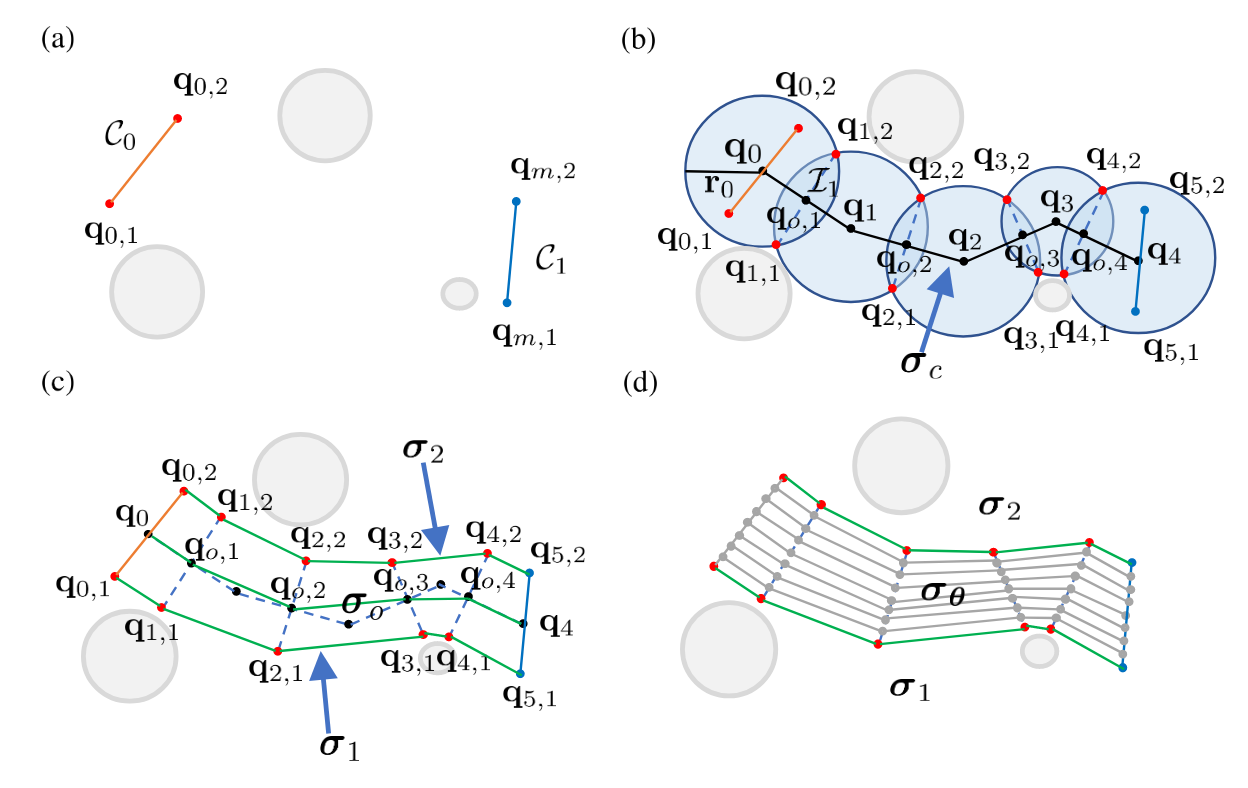
\includegraphics[scale=0.4]{img/tube.png}
	\caption{Diagram of Tube Generation}
	\label{fig1}
\end{figure}

2.Improved Progressive Goal Region Expansion

Since we have introduced a time dimension, it becomes challenging to generate samples distributed across the entire space if the time space is unbounded. However, applying any time constraint may render the planning problem unsolvable. Therefore, each time a new batch of samples is added, we gradually expand the sampling target area. To achieve this, we introduce several parameters: B.timeRange determines the time boundary, B.batchSize determines the number of samples generated after expansion. When a batch is filled, B.timeRange is increased by P.rangeFactor, and B.batchSize is adjusted accordingly. As the time boundary expands, due to the higher sample density at lower time values from previously generated samples, it becomes increasingly unlikely to find any solution. Hence, we employ weighted sampling to ensure a uniform distribution across the entire space.

3.Improved Conditional Sampling

Any state that can be part of the solution path must have a finite distance d from the starting point and at least one target state. Due to velocity constraints, only states at the intersection of the start cone and the target cone (see Figure 3) satisfy this requirement. Therefore, similar to informed RRT*, we only sample from the region where solutions can be generated. Ideally, sampling would directly occur from the union of the start velocity cone and the target velocity cone.

However, since it's not feasible to explicitly compute the intersection when there are multiple target states, we first uniformly sample a configuration c (Line 2 in Algorithm 5). Then, using c, we sample a feasible time within the possible time range restricted to c. The possible time range depends on $s_{start}$ and previously sampled target states. To achieve a more uniform sampling, we utilize two sets of target states: B.goals and B.newGoals. The time boundaries $t_{lb}$and $t_{ub}$ are obtained from the minimum arrival time from the starting configuration $c_start$ to c (Line 3) and the given maximum valid time.

\begin{algorithm}[H]
	\caption[short]{SampleConditionally}
	\begin{algorithmic}[1]
		\Input{$s_{start},\mathcal{Q},B$}
		\WHILE{}
		\STATE{$q \gets SampleUniform(\mathcal{X})$}
		\STATE{$t_{\min} \gets t_{start}+LowerBoundArrivalTime(q_{start},q)$}
		\IF{$Rand(0,1) \leq B.batchProbability$}
		\STATE{$t_{lb} = t_{\min}$}
		\STATE{$t_{ub} = MaxValidTime(q,B.goals)$}
		\ELSE{}
		\STATE{$t^*_{\min} = MaxValidTime(q,B.goals)$}
		\STATE{$t_{lb} = Max(t_{\min},t^*_{\min})$}
		\STATE{$t_{ub} = MaxValidTime(q,B.newgoals)$}
		\ENDIF{}
		\ENDWHILE{}
	\end{algorithmic}
\end{algorithm}

\subsection{reformulation dynamic coorid minimum snap Trajectory Optimization}
For the state sequence generated by TubeST-RRT*, trajectory optimization can be applied to make the trajectory smoother. In minimum snap trajectory optimization, the optimized trajectory needs to pass through intermediate path nodes. However, since our TubeST-RRT* incorporates collision detection within the spherical regions, it essentially provides a collision-free flight corridor. Therefore, the trajectory only needs to stay within this corridor to ensure collision-free movement. Traditional minimum snap optimization using polynomial parameters as optimization variables may lead to numerical instability when there are too many nodes. Here, we can use reformulation minimum snap to transform the optimization variables from polynomial coefficients to physically meaningful variables such as position ($p$), velocity ($v$), and acceleration ($a$). Constraints can be added to $p$ to ensure it stays within the circles generated by the planner. This ensures that the optimized trajectory is collision-free.

Input as

\begin{equation}
	s = [s_{0},s_{1},s_{2},\cdot{}\cdot{}\cdot{},s_{N}]
\end{equation}
where,$s_{i} = [x_{i},y_{i},z_{i},v_{yi},v_{zi},t_{i},r_{i}]$

A quintic polynomial is used to fit a uniaxial trajectory.
\begin{equation}
	\boldsymbol{p}\left( {t}\right)= {p}_{0} {t}^{0}+ {p}_{1} {t}^{1}+\cdots+ {p}_{5} {t}^{5}
\end{equation}

For the $N+1$ points generated by the planner (including the start point and the end point), it can be assumed that there are $N$ segments of the trajectory, where each segment of the trajectory is a higher-order polynomial, for minimum snap, our cost function is

\begin{equation}
	J= J_{1}+J_{2}+\cdots+J_{N} = \sum_{n=0}^M p_{m}^\top Q_{m}p_{m}
\end{equation}
where,$J_{m} = \int^{T_{m}}_{{T_{m-1}}}\left( \frac{d^4p(t)}{dt^4} \right)^2$

However, as the polynomial coefficients do not have practical physical meanings, when N is large, or in some special cases, this optimization problem can easily become numerically unstable, leading to difficulties in solving. To address this issue, a reformulation method was proposed to map the optimization variables to the physically meaningful variables $(p,v,a)$.

\begin{equation}
	\begin{align}
		\boldsymbol{A}_i\boldsymbol{p}_i=\boldsymbol{d}_i,\quad \boldsymbol{A}_i=\begin{bmatrix}\boldsymbol{A}_0\\\boldsymbol{A}_T\end{bmatrix}_i,\boldsymbol{d}_i=\begin{bmatrix}\boldsymbol{d}_0\\\boldsymbol{d}_T\end{bmatrix}_i
	\end{align}
\end{equation}
The mapping relationship between the polynomial coefficients and the motion differential has been obtained.
\begin{equation}
	\begin{align}
		& \boldsymbol{d}_{i}
		= 
		\boldsymbol{A}_{i} 
		\boldsymbol{p}_{i} \\
		& \boldsymbol{p}_{i} = \boldsymbol{A}_{i}^{-1}\boldsymbol{d}_{i}
	\end{align}
\end{equation}


% \begin{verbatim}
% \begin{figure}
%   \centering
%   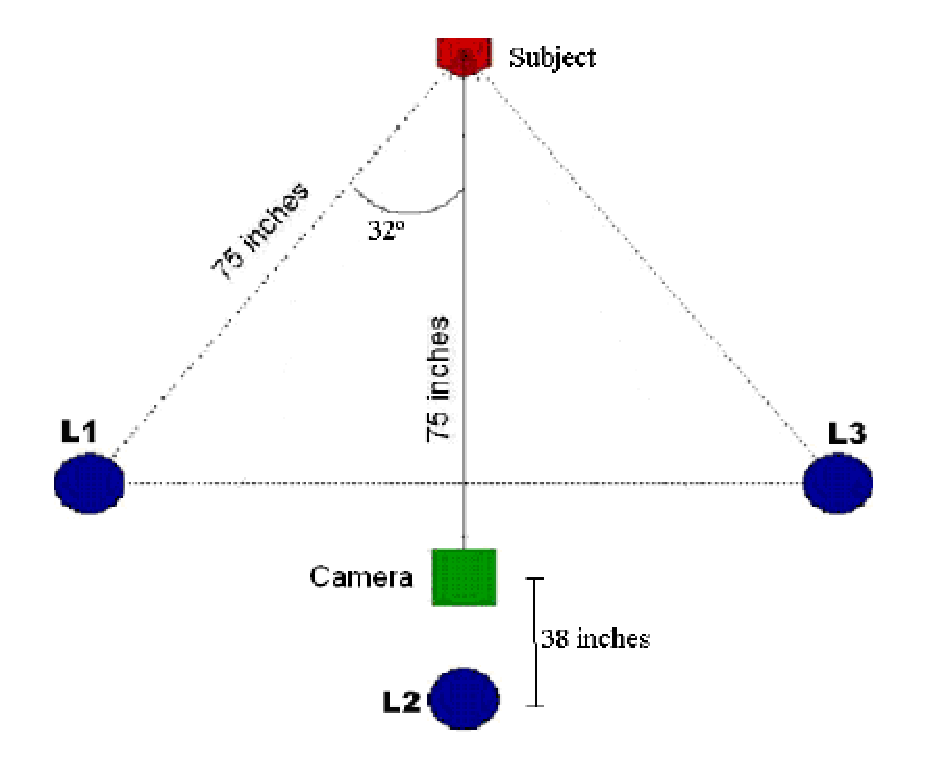
\includegraphics[scale=0.5]{fig01}
%   \caption{Write the figure caption here.}
%   \label{fig:pendulum}
% \end{figure}
% \end{verbatim}

% \begin{figure}
% 	\centering
% 	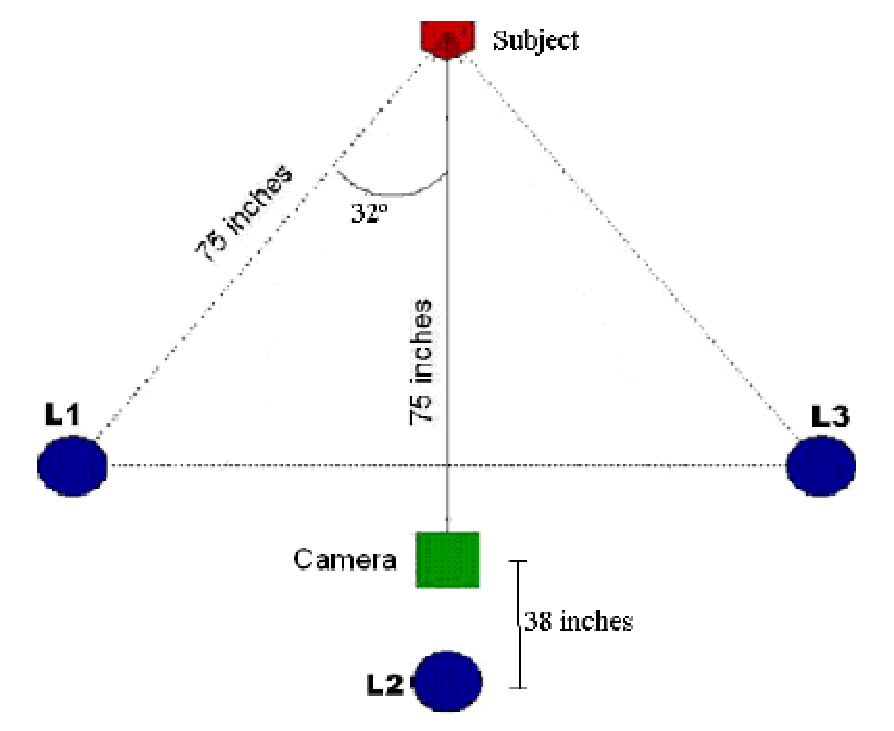
\includegraphics[scale=0.5]{fig01.pdf}
% 	\caption{Write the figure caption here.}
% 	\label{fig:pendulum}
% \end{figure}

% \subsection{And a table?}
% Just replace the text/values in the template table below
% with your own. You can change the number of
% lines/rows as necessary.

% \begin{table*}
% 	\centering
% 	\caption{Title of the table should be at the top}
% 	\begin{tabular}{|l|l|l|l|}
% 		\hline
% 		Column Name1    & Column Name2 & Column Name3 & Column Name4 \\
% 		\hline
% 		Parameter Name1 & Value        & Value        & Value        \\
% 		\hline
% 		Parameter Name2 & Value        & Value        & Value        \\
% 		\hline
% 		Parameter Name3 & Value        & Value        & Value        \\
% 		\hline
% 	\end{tabular}
% \end{table*}

% \subsection{Equations}
% Conventionally, in mathematical equations, variables and
% anything that represents a value appear in italics.
% All equations should be numbered for easy referencing.
% The number should appear at the right margin.
% \begin{eqnarray}
% 	S'_{\mathrm{pg}} = \frac{S_{\mathrm{pg}} - \mathrm{min}(S_{\mathrm{pG}})}
% 	{\mathrm{max}(S_{\mathrm{pG}} - \mathrm{min}(S_{\mathrm{pG}}))}
% \end{eqnarray}
% In mathematical expressions
% in running text "/" should be used
% for division (not a horizontal line).



\section{Citations}

Citations in the text can be made using\\[6pt]
\verb+\citet{NewmanGirvan2004}+\\[6pt]
for citation in running text like in
\citet{NewmanGirvan2004} or using\\[6pt]
\verb+\citep{Vehlowetal2013,NewmanGirvan2004}+\\[6pt]
for citation within parentheses like in
\citep{Vehlowetal2013,NewmanGirvan2004}.

Please use the actual \verb+\cite+ command in the text.
Also, please double-check the \verb+\citep+ command.

\section{Reference style}
You can include the references in the main text file in \LaTeX
format. Alternately, you can include a separate bibliography
file (refs.bib in this example) and run the following set of
commands:
\begin{verbatim}
  ==================

  pdflatex jasr-template.tex

  bibtex jasr-template (no extension in this line!)

  pdflatex jasr-template.tex

  pdflatex jasr-template.tex

  ==================
  \end{verbatim}

\section{A sample entry in the bibliography file}
%{\fontsize{7.5pt}{9.6pt}\selectfont
\begin{verbatim}
  ==================

  @ARTICLE{NewmanGirvan2004,
    author  = {Newman, M. E. J. and Girvan, M.},
    title   = {Finding and evaluating community 
                structure in networks},
    journal = {Phys. Rev. E.},
    volume  = {69},
    number  = {21},
    year    = {2004},
    pages   = {026113}
  }

  ==================
  \end{verbatim}
%}

\section*{Acknowledgments}
Acknowledgments should be inserted at the end of the paper,
before the references, not as a footnote to the title. Use the
unnumbered Acknowledgements Head style for the Acknowledgments
heading.

%% Bibliography
%% Author year style
\bibliographystyle{jasr-model5-names}
\biboptions{authoryear}
\bibliography{refs}

\end{document}

%%

